\chapter{Neurogenetic Programming}\label{ch:neurogen}
\begin{remark}
    An earlier revision of this chapter \cite{liventsev2021neurogenetic,liventsevNeurogeneticProgrammingFramework2021} was presented at GECCO 2021
\end{remark}

\section{Motivating example: neurogenetic optimization}

\paragraph{Gradient-free optimization}

Consider the task of finding the maximum of a function without any access to its derivative. For instance,

\begin{equation}
\obj(\mlinput) = \sin \mlinput + \sin 10 \mlinput - 0.01 \mlinput^2
\end{equation}

Using methods from single variable calculus \cite{antonCalculusSingleVariable2021}, one can derive the gradient of this function analytically:

\begin{equation}
\obj'(\mlinput) = \cos \mlinput + 10 \cos 10 \mlinput - 0.02 \mlinput
\end{equation}

However, a lot of functions we would like to optimize in real life (phone battery life, travel time, QALYs \cite{ryenWillingnessPayfitness2015, torranceUtilitiesfitnessadjustedLife1989}, profits) do not have a formula attached. 
So, for this thought experiment, consider $ \obj(\mlinput) $ as an opaque function to be explored only via querying the values of $ \obj(\mlinput) $ for some $\mlinput$.
This function is visualized on figure \ref{fig:neuropt-f}
    
\begin{figure}
    \centering
    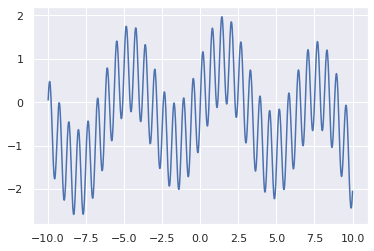
\includegraphics[width=0.8\linewidth]{images/neuropt1.png}
    \caption{$\obj(\mlinput)$}
    \label{fig:neuropt-f}
\end{figure}

The goal is to find $ \arg\max_\mlinput \obj(\mlinput) $

\paragraph{Evolutionary approach}

Let us begin with an intitial population of 2 instances of $ \mlinput $ and, At every iteration of the evolutionary algorithm, draw $ x_1 $ and $ x_2 $ from the exponential reward distribution $\prob(\mlinput) \sim e^{\obj(\mlinput)}$ and add $ \frac{x_1 + x_2}{2} $ to the population.
This offspring sampling procedure is repeated for 10000 iterations and from the resulting population of 10002 pick $ \mlinput $ with the maximal $ \obj(\mlinput) $.

By generating new solutions as modifications of existing successful solutions we focus the search on the most promising part of the search space. 
Note that the darker colored points of the visualization on figure \ref{fig:neuropt-search} were added to the population after the light colored ones. 

\begin{figure}
    \centering
    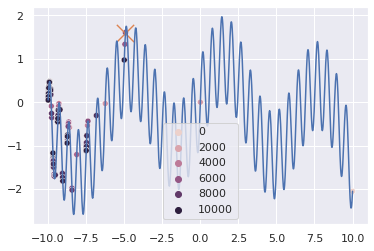
\includegraphics[width=0.8\linewidth]{images/neuropt2.png}
    \caption{Rollout of evolutionary optimization. The cross denotes the final solution}
    \label{fig:neuropt-search}
\end{figure}

One can see that 10000 iterations were not enough to find the highest peak, although the one we finally found is close. Most of the iterations were spent navigating the far left part of the search space. 
The right half of the search space remained unexplored - the rightmost solution $ \mlinput_\text{right} $ has an $ \obj(\mlinput_\text{right})=-2 $ which means it's almost never drawn from $ \prob(\mlinput) $. 
This could be mitigated by various means, for instance, \emph{temperature sampling} \cite{holtzman2019curious}, namely, adding a temperature parameter to $ \prob(\mlinput) $: $\policy_t(\mlinput) \sim e^{t\obj(\mlinput)}$.
But the issue is fundamental to evolutionary algorithms - a few unrepresentative examples can erroneously exclude a large part of the search space.

\paragraph{Neural Actor-Critic approach}

In the deep learning approach we train a \emph{critic} neural network $ \obj_{\learnables}(\mlinput) $ to mimic $ \obj(\mlinput) $ as closely as possible. Then all we need is a second neural network that represents a probability distribution of $ \mlinput $s that have a high $ \obj(\mlinput) $ and sample from it. It is called the \emph{actor} network, $ \mlinput_{\learnables}(\latent) $, representing a mapping from the normal distribution to the distribution of points with high $ \obj(\mlinput) $. See actor-critic methods in Reinforcement Learning \cite[section 13.5]{suttonReinforcementLearningSecond2018}.

We start with an empty population and, at every step, sample $ \latent $ from $ \normaldistr(0,1) $, add $ \mlinput_{\learnables}(\latent) $ to the population and update both $ \obj_{\learnables}(\mlinput) $ and $ \mlinput_{\learnables}(\latent) $. See figure \ref{fig:neuropt-actor-critic} for the resulting rollout.
    
\begin{figure}
    \centering
    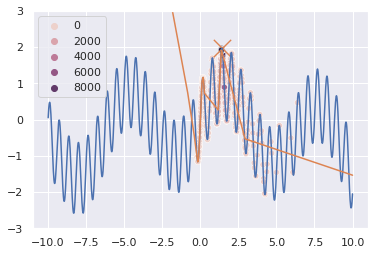
\includegraphics[width=0.8\linewidth]{images/neuropt3.png}
    \caption{Rollout of actor-critic optimization. $ \obj(\mlinput) $ in blue, $ \obj_{\learnables}(\mlinput) $ in orange}
    \label{fig:neuropt-actor-critic}
\end{figure}


\paragraph{Neurogenetic approach}

    
\begin{figure}
    \centering
    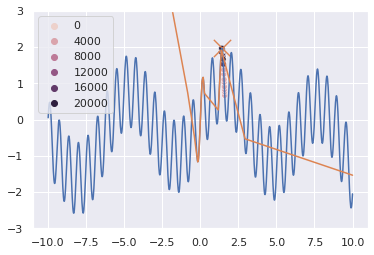
\includegraphics[width=0.8\linewidth]{images/neuropt4.png}
    \caption{Rollout of neurogenetic optimization. $ \obj(\mlinput) $ in blue, $ \obj_{\learnables}(\mlinput) $ in orange}
    \label{fig:neuropt-combined}
\end{figure}

Now, what if we alternate between neural steps and genetic steps?
On figure \ref{fig:neuropt-combined} we do exactly that: add one element to the population by sampling it from the actor distribution $ \mlinput_{\learnables}(\latent) $, update the actor and the critic, then sample a pair $\langle x1,x2 \rangle$ as we did in the evolutionary approach and add their average.
One can see that in the hybrid neural-genetic mode, the search process zeros in on the maximum really fast and finds it within 4000 iterations, faster than both pure neural and pure genetic approaches 

\newpage
\section{From Neurogenetic Optimization to Neurogenetic Programming}

In \emph{genetic programming} \cite{genprog1,genprog2} new programs are generated by mutating and mixing a \emph{population} of programs. 
 A more recent approach, largely drawing on the earlier success of deep neural language models (see CodeBERT \cite{codebert} inspired by BERT \cite{devlinBERTPretrainingDeep2019}), have been to train black box \emph{neural models} that generate executable programs as text \cite{abolafiaNeuralProgramSynthesis2018,deepcoder,structural}. 
 Neural program synthesis and genetic programming both have unique advantages \cite{geneticvsneural}. 
 In this chapter we propose a novel hybrid of the two families of methods. We call the method \emph{Instant Scrum} in reference to a popular Agile software team work model \cite{scrum}. We show that \emph{Instant Scrum}, IS, can solve several reinforcement-guided program synthesis tasks in standard OpenAI gym benchmarks tasks (section \ref{sec:tasks}). 

After the introduction to the relevant background in the next section, we will give a detailed description of the proposed IS methodology. Next, we describe the experimental setup and the OpenAI gym test tasks, and the results of the experiments in several variations of the core IS method. Finally, we discuss the results and propose future research directions and potential applications for hybrid neurogenetic programming. 

This chapter is dedicated to answering \rqneurogen:

\begin{highlight}
    Can neurogenetic program synthesis improve upon neural program synthesis with BF++?
\end{highlight}

\newpage
\section{Instant Scrum}

\begin{remark}
    An implementation of Instant Scrum is available as part of Cibi \cite{liventsevVadim0x60Cibi2024} package
\end{remark}

How does one manage a composition of code generators in such a way that the composition yields better programs than individual contributors are capable of? 
This question is studied extensively in software project management literature \cite{mythicalmanmonth}.
And while, admittedly, project management literature is concerned with human developers and, admittedly, there exist considerable differences between human developers and mathematical models of code generation \cite{bugfixing}, we mitigate these differences with several simplifying assumptions.

\subsection{Modeling the codebase}

Following from traditional genetic programming, we define a \emph{population} of programs. 
The \emph{codebase} is a tuple of 2-tuples, representing each program $\code_\step$ and the total reward it collected $\returntot^\step$ (see section \ref{sec:fitness}):

\begin{equation}
    \codebase = \langle \langle \code_1, \returntot^{(1)} \rangle, \langle \code_2, \returntot^{(2)} \rangle \dots \langle \code_{|\codebase|}, \returntot^{(|\codebase|)} \rangle \rangle
\end{equation}

where $|\codebase|$ is the number of elements in $\codebase$.
However, unlike in traditional genetic programming, the \emph{initial population} can (optionally) be empty.
Note that the same program may occur in the population multiple times, possibly with different values of $\returntot$, since the evaluation environment can be stochastic.

\subsection{Modeling a software developer}
\label{sec:developer}

A software developer can:
\begin{enumerate}
    \item Check out programs from the codebase $\codebase$
    \item Output new a program $\code$
    \item Receive feedback on their program's fitness $\obj$ 
    \item Learn from the feedback by modifying its strategy
\end{enumerate}

Thus, a developer is a 2-tuple of a program distribution $\policy_\text{dev}(c | \learnables, \codebase)$ and a parameter update procedure $\mathit{Update}(\learnables, \code, \obj)$

Distribution $\policy_{\text{dev}}(c | \learnables, \codebase)$ is defined over programs and is parametrized with learnable parameters $\learnables$ as well as codebase $\codebase$. 
Having codebase as parameter enables the developer to generate new programs as a modification and/or combination of existing programs, i.e. to apply genetic programming.

Learnable parameters $\learnables$ encode the developer's current methodology of programming that can be modified upon receipt of positive or negative feedback using the developer's update procedure. 

The \emph{team} of developers is a tuple of 2-tuples:
\begin{equation}
    \team = \langle \langle \team_p^{(1)}, \team_\text{upd}^{(1)} \rangle, \langle \team_p^{(2)}, \team_\text{upd}^{(2)} \rangle \dots \langle \team_p^{(|\team|)}, \team_\text{upd}^{(|\team|)} \rangle \rangle
\end{equation}

\newpage \subsection{Modeling program fitness}
\label{sec:fitness}

We define two empirical metrics of overall program fitness.
The first is \emph{empirical total reward}:

\begin{equation}
    \reward(\code|\codebase) = \frac{\sum\limits_{\step=1}^{|\codebase|} \mathbb{I}[\code_\code^{(\step)}=\code] \returntot^{(\step)}}{\sum\limits_{\step=1}^{|\codebase|} \mathbb{I}[\code_\code^{(\step)}=\code]}
\end{equation}

If a program has been tested in the environment ($\textit{Eval()}$ function) several times, there will be several copies of it in the codebase with different fitness samples.
Averaging over them yields an unbiased estimate of $\expectation(\returntot)$, the reinforcement learning objective.

The second is \emph{empirical program fitness}, defined as

\begin{equation}
    \obj(\code|\codebase) = \frac{\sum\limits_{\step=1}^{|\codebase|} \mathbb{I}[\codebase_\code^{(\step)}=\code] e^{\returntot^{(\step)}}}{\sum\limits_{\step=1}^{|\codebase|} \mathbb{I}[\code_\code^{(\step)}=\code]}
    \label{eq:empfitness}
\end{equation}

\emph{Empirical program fitness} is an unbiased estimate of $\mathbb{E}(e^{\mathit{Eval}(\code)})$
The idea behind exponentiating the total reward is to encourage \emph{exploration} \cite{exploration}.
Programs that on average perform poorly, but sometimes, stochastically, collect high rewards, will have a higher $\obj(\code|\codebase)$ than $\reward(\code|\codebase)$.
We consider these programs to be \emph{high-fitness additions to the codebase} because they contain the knowledge necessary for solving environment $M$, even if on average they do not solve it.
We hypothesize that applying \emph{genetic operators} (section \ref{sec:genetic}) to programs with high $\obj(\code|\codebase)$ can yield programs with high $\reward(\code|\codebase)$.
For this reason we train developers to maximize $\obj$, but when the training is complete, we pick programs from the codebase with the highest $\returntot$ as "best programs".
 
$\obj(\code|\codebase)$ has an additional technical advantage over $\reward(\code|\codebase)$: invariant $\obj(\code|\codebase) \geq 0$ holds for all $\code$.
This lets one sample programs from the codebase with probabilities proportional to their fitness, see eq. \ref{eq:genmixture}.

\newpage \subsection{Populating the codebase}

Just like \emph{instant run-off voting} achieves similar results to \emph{exhaustive ballot runoff voting}, but does it much faster by replacing a series of ballots cast in a series of elections with a ballot cast once that goes on to participate in a series of virtual elections \cite{votingsystems}, our \emph{Instant Scrum} algorithm does the same to Scrum \cite{scrum}: it simulates the iterative software development process recommended by Scrum methodology without humans in the loop making it possible to run many sprints per second:

\begin{algorithm}[H]
\begin{algorithmic}[1]
\caption{Instant Scrum with a team of developers}
\label{alg:instantscrum}
\Procedure{InstantScrum}{$T,\codebase,N_\text{max}$}
\State $N \gets 0$
\While{$N < N_\text{max}$}
\LineComment{For each developer in the team}
\For{$\step = 1,2,\dots,\team$}
\LineComment{Sample a program from the developer}
\State $\code_\text{new}\sim \policy_i(\code | \learnables_i, \codebase)$ 
\LineComment{Test the program}
\State $\returntot \gets \mathit{Eval}(\code_\text{new})$
\LineComment{Save the code and test result to the codebase}
\State $\codebase \gets \codebase \cup \{\langle \code_\text{new}, \returntot \rangle\}$
\LineComment{Train the developer}
\State $\mathit{Update}_i(\learnables_i, \code, \obj)$
\LineComment{Increment sprint counter}
\State $N \gets N+1$
\EndFor
\EndWhile
\EndProcedure
\end{algorithmic}
\end{algorithm}

To combine genetic programming and neural program synthesis we introduce 3 types of developers: \emph{genetic} and \emph{neural} and \emph{dummy}, create a team $\team$ that contains developers of all types and run \emph{Instant Scrum}.

\newpage \subsection{Genetic developers}
\label{sec:genetic}

A genetic developer writes programs by
\begin{enumerate}
    \item Selecting one of the 7 available stochastic \emph{genetic operators} (described below)
    \item Selecting two programs from the \emph{codebase} $\codebase$ (parents $\code_1$ and $\code_2$) 
    \item Using the operator to modify the parents and yield a new (child) program
\end{enumerate}

A genetic operator is a probability distribution $\policy_\text{op}$ over child programs given 2 parent programs. 

\begin{equation}
    \policy_\text{op}(\code_\text{child}|\code_1,\code_2)
\end{equation}

Operators whose $\policy_\text{op}$ is invariant to $\code_2$ and depends on $\code_1$ only are called \emph{mutation} operators: they generate a new program by \emph{mutating} one program $\code_1$.
The rest are called \emph{combination} operators as they \emph{combine} 2 existing programs to generate a new one.
The choice of operators follows from DEAP \cite{deap, derainvilleDEAPEnablingNimbler2014, derainvilleDEAPPythonFramework2012} which we also use to implement the experiments.

\paragraph{Mutation operators}

The simplest method for randomly modifying a program is \emph{shuffle mutation}: randomly re-order the tokens of $\code_1$.
Let $\mathrm{A}$ be the set of all possible permutations of size $|\code_1|$. $|\mathrm{A}|=|\code_1|!$. 
Then

\begin{equation}
    \policy_\text{shuffle}(\code_\text{child}|\code_1,\code_2) =
            \frac{\sum\limits_{\action \in \mathrm{A}} \mathbb{I}[\action(\code_\text{parent}) = \code_\text{child}]}{|\code_1|!}
\end{equation}

Another approach is \emph{uniform mutation} where a loaded coin is tossed for every token in $\code_1$. 
With probability $\policy_\text{ind}$ it is replaced with a random token from the alphabet $\alphabet$ of the programming language, with probability $1-\policy_\text{ind}$ it stays the same.
The evolution of a single token under shuffle mutation is defined by distribution

\begin{equation}
    \prob(\code^\text{new} | \code^\text{old}) = \frac{\policy_\text{ind}}{|L|} +  (1 - \policy_\text{ind}) \mathbb{I}[\code^\text{new} = \code^\text{old}]
\end{equation}

Hence over full programs the operator is defined as

\begin{equation}
    \policy_\text{unimut}(\code_\text{child}|\code_1,\code_2) = \mathbb{I}[|\code_\text{child}|=|\code_1|] \\ 
    \prod\limits_{\step=0}^{|\code_1|}  \left(\frac{\policy_\text{ind}}{|L|} +  (1 - \policy_\text{ind}) \mathbb{I}[\code_\text{child}^{(\step)} = \code_1^{(\step)}] \right)
\end{equation}

\paragraph{Combination operators}

The combination operators we propose are all variants of \emph{crossover} - a classic genetic programming technique rooted in the way a pair of DNA molecules exchanges genes during mitosis and meiosis.

In DNA \cite{evocritique}, as well as in most genetic programming literature \cite{genprog1,genprog2} the crossover operator combines 2 parent sequences to produce 2 children.
In this section, in order to reduce complexity, we define the distributions as if only the first child program is saved and the second one is forgotten.
Since program pair $\langle \code_2, \code_1 \rangle$ is equally likely to be selected for combination as $\langle \code_1, \code_2 \rangle$ (see eq. \ref{eq:genmixture}) this modification does not affect the resulting genetic developer distribution.

In \emph{one-point crossover} a random cut position $k$ is selected and the trailing sections of 2 parent programs beginning with the cut point are swapped with each other. 
If the parent programs have different lengths, the cut point has to fit within both programs:

\begin{equation}
    2 \leq k \leq |\code_1,\code_2|; |\code_1,\code_2| = \min\{|\code_1|, |\code_2|\}
\end{equation}

Hence the probability of $\code_\text{child}$ being born out of \emph{one-point crossover} is

\begin{equation}
    \policy_\text{1ptcx}(\code_\text{child}|\code_1,\code_2) =
        \frac{\mathbb{I}[|\code_\text{child}|=|\code_2|]}{|\code_1,\code_2|-1}
        \sum\limits_{k=2}^{|\code_1,\code_2|} \prod\limits_{\step=1}^{k-1} \mathbb{I}[\code_\text{child}^{(\step)} = \code_1^{(\step)}] \prod\limits_{\step=k}^{|\code_2|} \mathbb{I}[\code_\text{child}^{(\step)} = \code_2^{(\step)}]
\end{equation}

\emph{Two-point crossover} is similar, but instead of swapping the trailing ends of programs, a section in the middle of the programs is chosen, determined by randomly selected cut-off indices $k_1$ and $k_2$ and swapped:

\begin{multline}
    \policy_\text{2ptcx}(\code_\text{child}|\code_1,\code_2) =
        \frac{2 \mathbb{I}[|\code_\text{child}|=|\code_1|]}{(|\code_1,\code_2|-2)(|\code_1,\code_2|-1)} 
        \cdot \\ \cdot
        \sum\limits_{k_1=2}^{|\code_1,\code_2|-1}
        \sum\limits_{k_2=k_1+1}^{|\code_1,\code_2|} 
        \prod\limits_{\step=1}^{k_1-1} \mathbb{I}[\code_\text{child}^{(\step)} = \code_1^{(\step)}] \prod\limits_{\step=k_1}^{k_2-1} \mathbb{I}[\code_\text{child}^{(\step)} = \code_2^{(\step)}]
        \prod\limits_{\step=k_2}^{|\code_1|} \mathbb{I}[\code_\text{child}^{(\step)} = \code_1^{(\step)}]
\end{multline}

\emph{Uniform crossover} mirrors \emph{uniform mutation} in that a loaded coin is tossed for each token in $\code_1$. With probability $\policy_\text{ind}$ the token is replaced, but the replacement is not drawn randomly from the alphabet. Instead, the replacement comes from $\code_2$:

\begin{equation}
    \policy_\text{unicx}(\code_\text{child}|\code_1,\code_2) = \prod\limits_{\step=0}^{|\code_1|} \mathbb{I}[|\code_\text{child}|=|\code_1|] \\ \left(\policy_\text{ind} \mathbb{I}[\code_\text{child}^{(\step)} = \code_2^{(\step)}] + (1 - \policy_\text{ind}) \mathbb{I}[\code_\text{child}^{(\step)} = \code_1^{(\step)}] \right)
\end{equation}

Finally, \emph{messy crossover} is a version of \emph{one-point crossover} without the assumption that both parent programs have to be cut at the same index $k$.
In \emph{messy crossover}, one parent is cut at index $k_1$, another is cut at index $k_2$ and the head of one is attached to the tail of the other:

\begin{multline}
    \policy_\text{messy}(\code_\text{child}|\code_1,\code_2) = \frac{1}{(|\code_1,\code_2|-1)^2} \cdot \\ \cdot \sum\limits_{k_1=2}^{|\code_1,\code_2|} \sum\limits_{k_2=2}^{|\code_1,\code_2|} \mathbb{I}[|\code_\text{child}|=k_1+|\code_2|-k_2] \prod\limits_{\step=1}^{k_1-1} \mathbb{I}[\code_\text{child}^{(\step)} = \code_1^{(\step)}] \prod\limits_{\step=1}^{|\code_2|-k_2} \mathbb{I}[\code_\text{child}^{(k_1+\step)} = \code_2^{(k_2+\step)}]
\end{multline}

\begin{table}
    \centering
    \begin{tabular}{r|l}
         Parent 1 & \color{blue}\verb|ae>>>>>34+| \\
         Parent 2 & \color{red}\verb|a[e>-a-]b[e>>-b-]| \\
         \midrule
         Shuffle mutation & \color{blue}\verb|>>4+>3>e>a| \\
         Uniform mutation & \color{blue}\verb|ae|\color{black}\verb|@|\color{blue}\verb|>|\color{black}\verb|!|\color{blue}\verb|>>3|\color{black}\verb|5|\color{blue}\verb|+| \\
         1-point crossover & \color{blue}\verb|ae>>>>|\color{red}\verb|-]b[e>>-b-]| \\
         2-point crossover & \color{blue}\verb|ae>|\color{red}\verb|>-a-|\color{blue}\verb|34+| \\
         Uniform crossover & \color{blue}\verb|ae|\color{red}\verb|e|\color{blue}\verb|>|\color{red}\verb|-|\color{blue}\verb|>>3|\color{red}\verb|b|\color{blue}\verb|+| \\
         Messy crossover & \color{blue}\verb|ae>>>>|\color{red}\verb|e>-a-]b[e>>-b-]| \\
         Pruning & \color{blue}\verb|e>>>>>4+| \\
    \end{tabular}
    \caption{All operators applied a pair of BF++ programs}
\end{table}


\paragraph{Pruning operator}

After initial experiments  we found that generated programs often contain sections of unreachable code or code that makes changes to the execution state and fully reverses them.
To address this, we introduced an additional operator for removing dead code (\emph{pruning}): when Instant Scrum encounters a successful program, pruning helps separate sections of this program that led to its success from sections that appeared in a highly-rated program by accident.  

Implementation of the pruning operator depends on the programming language at hand, here we define it as a pruning function $\code_\text{pruned}=\mathit{Prune}(\code_1)$ that outputs a program functionally equivalent to $\code_1$ (memory functions $(\action,\memory)$ of $\code_\text{pruned}$ are equal to that of $\code_1$) and $|\code_\text{pruned}| \leq \code_1$ and a degenerate probability distribution:

\begin{equation}
    \policy_\text{prune}(\code_\text{child}|\code_1,\code_2)= \begin{cases}
        1 & \code_\text{child} = \mathit{Prune}(\code_1) \\
        0 & \text{otherwise}
        \end{cases}
\end{equation}

\newpage
\paragraph{Operator and parent selection}

Let $\probs_\text{genetic}$ be a tuple of all available genetic operators, in order of introduction, i.e. $\probs_\text{genetic}^{(1)}=\policy_\text{shuffle}$ and $\probs_\text{genetic}^{(4)}=\policy_\text{2ptcx}$

Genetic developer's program distribution is a mixture distribution, combining different operators that can be applied, weighted by learnable parameters, and different programs that can be sampled from the codebase, weighted by \emph{empirical fitness} (eq. \ref{eq:empfitness}).

\begin{equation}
    \policy_\text{genetic}(\code | \learnables, \codebase) = 
    \sum\limits_{\code_1}^{\codebase}  
    \sum\limits_{\code_2}^{\codebase} 
    \frac{\obj(\code_1|\codebase) \obj(\code_2|\codebase)}{(\sum\limits_{\code}^{\codebase} \obj(\code|\codebase))^2} 
    \sum\limits_{\step=0}^{|\probs_\text{genetic}|} 
    \learnables_i \probs_\text{genetic}^{(\step)} (\code|\code_1,\code_2)
    \label{eq:genmixture}
\end{equation}

This is a true probability distribution if and only if $\sum\limits_{\step=0}^{|\probs_\text{genetic}|} 
    \learnables_i = 1$


\paragraph{Training the genetic developer}

One challenge that remains to be solved to fully define the genetic developer (following section \ref{sec:developer}) is to define a learning from feedback strategy $\mathit{Update}_\text{genetic}$.
To do this, we notice that equation \ref{eq:genmixture} contains a \emph{multi-armed bandit} \cite{banditproblem} hiding in plain sight.
Indeed, once the \emph{genetic} developer samples $\code_1$ and $\code_2$ from the codebase, it has to pick one of 7 available options (pull one of 7 \emph{levers}) to then receive a reward $\mathit{Eval}(\code_\text{child})$.
This subproblem can be represented with a POMDP of its own and solved using one of the standard bandit algorithms \cite{banditsolutions}.

Following \emph{Occam's razor}, we picked the simplest method, \emph{epsilon-greedy optimization}, where the value of each operator is mean total reward of programs generated with it:

\begin{equation}
    \statevalue^{(\step)} = \frac{1}{|\codebase(\probs_\text{genetic}^{(\step)})|} 
    \sum\limits_{k=1}^{|\codebase(\probs_\text{genetic}^{(\step)})|}
    \codebase(\probs_\text{genetic}^{(\step)})_R^{(k)} 
\end{equation}

where $\codebase(\probs_\text{genetic}^{(\step)})$ is the subset of the codebase produced via operator $\probs_\text{genetic}^{(\step)}$.

The $\mathit{Update}_\text{genetic}$ procedure recalculates values $\statevalue$ and sets operator probabilities to

\begin{equation}
    \learnables_i = \frac{\greed}{|\probs_\text{genetic}^{(\step)}|} +
    \mathbb{I}[\step = \underset{\step}{\arg\max} \statevalue^{(\step)}] (1 - \greed)
\end{equation}

where $\greed$ is a hyperparameter that controls the \emph{exploration-exploitation tradeoff} \cite{banditsexplo}

In future work, however, other bandit optimization algorithms can be used in its place \footnote{Our open-source software implementation allows for drop-in replacement of bandit algorithms}.

\paragraph{Hyperparameters}
\label{sec:genhyper}

The genetic developer, as described above, has 2 hyperparameters:

\begin{enumerate}
    \item $\policy_\text{ind}$ defines severity of mutation in $\policy_\text{unimut}$ and $\policy_\text{unicx}$
    \item $\greed$ defines learnability of genetic operator distribution
\end{enumerate}

Note that the \emph{team} mechanism afforded by \emph{Instant Scrum} can be used not only to combine genetic and neural program synthesis, but also to combine several genetic developers with different hyperparameters.

\newpage \subsection{Neural developers}
\label{sec:neural}

The \emph{neural developer}, also known as the \emph{senior developer} because of their unique ability to write original programs, is an LSTM \cite{hochreiterLongShorttermMemory1997} network followed by a linear layer that generates a sequence of vectors $\hidden_{1},\hidden_{2},\hidden_{3},\dots$ where $\hidden_i \in \realnums^{|\alphabet| + 1} \forall \step$ and $\stepp$-th element of vector $\hidden_i$, $\hidden_i^{(\stepp)}$, represents the probability of $\step$-th token of the program being $\stepp$-th token in the alphabet, $\prob(\code^{(\step)}=\alphabet^{(\stepp)})$.
The last element of the vector represents a special \emph{end of program} symbol.
This vector depends deterministically on the full set of neural network parameters (LSTM and linear layer) $\learnables$ and can be represented as a function $\hidden_i(\learnables)$.
Then

\begin{equation}
    \policy_\text{neural}(\code | \learnables, \codebase) = \hidden_{(|\code|+1)}^{\alphabet+1}
    \prod\limits_{\step=1}^{|\code|}
    \sum\limits_{j=1}^{|\alphabet|} \mathbb{I}[\code^{(\step)}=\alphabet^{(j)}]
    \hidden_i(\learnables)
\end{equation}

For the $\mathit{Update}_\text{neural}$ procedure we use the algorithm proposed in \cite{abolafiaNeuralProgramSynthesis2018}.
The subproblem of generating a program $\code$ is considered as a reinforcement learning episode of it's own, where tokens are actions and token number $|\code|+1$ (\emph{end of program} token) is assigned reward $\obj = e^\returntot; \returntot \sim Eval(\code)$. 
In this subenvironment $\hidden_\step(\learnables)$ is the policy network \cite[chapter 13]{suttonReinforcementLearningSecond2018} trained using REINFORCE algorithm with Priority Queue Training.
This algorithm involves a priority queue of best known programs: we implement it as programs from $\codebase$ with highest $\obj(\code|\codebase)$ which means that the neural developer can train on programs written by other developers.

$\hidden_i(\learnables)$ can also represent several LSTM layers stacked or a different type of recurrent neural network, i.e. GRU \cite{choPropertiesNeuralMachine2014,chung2014empirical}.
Hyperparameters of this neural network, such as hidden state size and/or number of stacked layers are hyperparameters of the neural developer.  

\newpage \subsection{Dummy developer}

The last developer we introduce is the simplest one:

\begin{equation}
    \policy_\text{dummy}(\code_\text{child}|\code_1,\code_2) = 
    \frac{\obj(\code_\text{child}|\codebase)}{\sum\limits_{\code}^{\codebase} \obj(\code|\codebase)} 
    \label{eq:dummy}
\end{equation}

Dummy developer does not generate novel programs.
Instead, it uses the same fitness-weighted program sampling as in equation \ref{eq:genmixture} to decide which existing program to copy.
Their utility may not be obvious at first, but note (section \ref{sec:fitness}) that when the same program is added to the codebase several times, it's total reward and fitness estimates are averaged and grow more accurate.

Dummy developer is a smart compromise between speed at which \emph{Instant Scrum} (algorithm \ref{alg:instantscrum}) is searching the program space and the fitness of its working map of the program space, focusing on its most "interesting" (high $\obj(\code|\codebase)$) parts. 
Without dummy developer, all empirical total rewards $E[Eval(\code)]$ would be low fitness estimates of true fitness of the program and one spurious success of an otherwise bad program could steer the search in the wrong direction.
On the other hand, we could test each program many times before adding it to the codebase, but that would slow down the search prohibitively. 

\newpage
\section{Experimental setup}
\label{sec:neurogen-experiments}

\paragraph{Teams}

In the table below, we introduce 5 teams.
Neural developers are denoted as lstm(hidden state dimensionality), several numbers mean a stacked LSTM.
Genetic developers are denoted as $\text{gen}(\policy_\text{ind},\greed)$, see section \ref{sec:genhyper}.
$\team_\text{small}$ and $\team_\text{large}$ are recommended configurations while $\team_\text{genetic}$, $\team_\text{neural}$ are \emph{ablation studies} to prove that combination of neural and genetic methods is useful.

\begin{table}[H]
\centering
\begin{tabular}{r|c|c|c|c}
     Developer & $\team_\text{small}$ & $\team_\text{large}$ & $\team_\text{genetic}$ & $\team_\text{neural}$  \\
     $\text{lstm}(10)$ & & \checkmark & & \\
     $\text{lstm}(50)$ & & \checkmark & & \\
     $\text{lstm}(256)$ & & \checkmark & & \\
     $\text{lstm}(10,10)$ & & \checkmark & & \\
     $\text{lstm}(50,50)$ & \checkmark & \checkmark & & \checkmark \\
     $\text{lstm}(256,256)$ & & \checkmark & & \\
     $\text{gen}(0.2,0.2)$ & \checkmark & &  & \\
     $\text{gen}(\frac{1}{3},0.2)$ & & \checkmark & & \\
     $\text{gen}(\frac{1}{6},0.2)$ & & \checkmark & & \\
     $\text{gen}(\frac{1}{12},0.2)$ & & \checkmark & & \\
     dummy & \checkmark & \checkmark & \checkmark & \checkmark \\
\end{tabular}
\caption{Team composition}
\end{table}


\paragraph{Language}

Instant Scrum can be used to generate programs in any programming language provided:
\begin{enumerate}
    \item An interpreter $\langle \action,\memory \rangle$, see section \ref{sec:rlcef}
    \item A known finite alphabet $\alphabet$
    \item A pruning function $\mathit{Prune}(\code)$
\end{enumerate}

The complexity of the chosen language is important since in complex languages random perturbations of program source code often produce grammatically invalid programs.
This issue has been addressed with \emph{structural models} \cite{grammargp,structural} \cite[chapter 4]{genprog1}, however, we sidestep the issue entirely by using \emph{BF++} (see chapter \ref{ch:bfpp}) - a simple language developed for \emph{reinforcement learning from code execution feedback} where most random combinations of characters are valid programs.
Each BF++ command is represented with a single character, thus the only way to tokenize it is to let tokens $\token_1,\token_2,\token_3,\dots$ be single characters.

\paragraph{Tasks}
\label{sec:tasks}

Following from the previous chapter we synthesize programs for \textbf{CartPole-v1} \cite{cartpole}, MountainCarContinuous-v0 (\textbf{MCC-v0}) \cite{mountain_car}, \textbf{Taxi-v3} \cite{taxi} BipedalWalker-v2 (\textbf{BW-v2})  Gymnasium \cite{towersGymnasiumStandardInterface2024} environments, see figure \ref{fig:envs}.

\paragraph{Initial populations}

Where possible, we run all experiments twice - a control experiment with empty intial codebase, and an experiment where codebase is pre-populated with human-written programs from chapter \ref{ch:bfpp}.
Exceptions to this rule are 
\begin{itemize}
    \item Teams $\team_\text{genetic}$ and $\team_\text{pure}$ that only have code modification (not generation) capability and thus require initialization 
    \item \textbf{BipedalWalker-v2} environment, because this environment proved challenging to manually develop BF++ for (see chapter \ref{ch:bfpp})
\end{itemize}

\paragraph{Stopping and scoring}

For Taxi we set an $N_\text{max}$ to $100000 \team$ sprints where $\team$ is the team size, meaning every developer in the team trains for 100000 iterations.
For other tasks we used Exponential Variance Elimination \cite{evestop} early stopping algorithm to stop the process when the positive trend in $\returntot$ is not present for 10000 sprints.
This approach rules out the hypothesis that \emph{Instant Scrum} is equivalent to enumerative search and it finds good programs by exhaustion as opposed to learning - if that was the case, early stopping would fire immediately.
Taxi environment is treated differently because programs that cannot pick up and drop off at least one passenger are always rewarded with -200 and at first it takes many iterations to synthesize at least one program that can.
In addition to these stopping rules, a hard timelimit was set.

After the process is stopped, we pick 100 programs with the highest $\returntot$ and make sure each of them has been tested at least 100 times, running additional evaluations if needed.

\newpage
\section{Results}
\label{sec:neurgen-results}

\begin{table*}[]
    \centering
    \begin{tabular}{c|c|c|c|c|c|c|c}
         Environment & \multicolumn{2}{c}{CartPole-v1} & \multicolumn{2}{c}{MCC-v0} & \multicolumn{2}{c}{Taxi-v3} & BW-v2 \\
         Initial programs & & 20.48 & & -6.55 & & -150.44 & \\
         \midrule
         $\team_\text{small}$  &    60.93 &    143.91 &     \textbf{92.53} &     88.20 &   -148.23 &   -150.44 &     -0.16\\
         $\team_\text{large}$ & \textbf{157.35} &     57.47 &     91.65 &     91.42 &    \textbf{-32.12} &   -150.44 &      \textbf{8.13} \\ 
         $\team_\text{genetic}$& - & 59.12 & - & 0 & - & -47.54 & - \\ 
         $\team_\text{neural}$ & 71.38 & 96.64 & 88.41 & 91.38 & -198.9 & -150.44 & 6.17 \\
         \midrule
         Leaderboard threshold & 195 & 195 & 90 & 90 & 0 & 0 & 300 \\ 
    \end{tabular}
    \caption{Averaged 100-episode reward acheived by the best program in each category}
    \label{tab:neurogenetic-results}
\end{table*}

See table \ref{tab:neurogenetic-results} for a summary of best programs generated.
The metric used, average $\returntot$ over 100 evaluations is the same metric that's used in the OpenAI gym leaderboard, so we include the threshold required to join the leaderboard for context.
\emph{Initial programs} refers to the best program in the codebase before \emph{Instant Scrum} starts when it is prepopulated with  programs from chapter \ref{ch:bfpp}.

Hybrid teams $\team_\text{small}$ and $\team_\text{large}$ perform significantly better than $\team_\text{genetic}$ and $\team_\text{neural}$, hence we can answer \rqneurogen positively: neurogenetic approach can be superior to neural program induction or genetic programming separately.

Besides, one unintuitive result of our experiments is that initialization of the codebase with previously available programs can be harmful, see $\team_\text{large}$.
Overall, best results were acheived without inspiration from human experts, however, it is very valuable for lightweight teams with few small (in terms of $|\learnables|$) developers.

Additionally, we can examine in more detail how single developers compare to each other (and notice that only neural developers are on the list): 

\begin{table}[H]
\centering
\begin{tabular}{r|c|c|l}
    Task & Init & $\reward(\code|\codebase)$ & Developer \\
    \midrule
    CartPole-v1 & & 157.35 & lstm(256) \\
CartPole-v1 & \checkmark & 57.47 & lstm(256,256) \\
MountainCar & & 91.65 & lstm(10,10) and pruning \\
MountainCar & \checkmark & 91.42 & lstm(50) \\
Taxi-v3 & & -32.12 & lstm(50) \\
Taxi-v3 & \checkmark &  -150.44  & human \\
BipedalWalker-v2 & & 8.13 & lstm(256,256) \\
\end{tabular}
\caption{Members of $\team_\text{large}$ that generated the best program}
\end{table}

The same is true for $\team_\text{small}$:

\begin{table}[H]
\centering
\begin{tabular}{r|c|c|l}
    Task & Init & $\reward(\code|\codebase)$ & Developer \\
    \midrule
    CartPole-v1 & & 60.93 & lstm(50,50)  \\
CartPole-v1 & \checkmark & 143.9 & lstm(50,50) \\
MountainCar & & 92.53 & lstm(50,50) \\
MountainCar & \checkmark & 88.2 & lstm(50,50) \\
Taxi-v3 & & -148.23 & $\text{gen}(0.2,0.2)$, $\policy_\text{unicx}$ \\
Taxi-v3 & \checkmark & -150.44 & human \\
BipedalWalker-v2 & & -0.15 & lstm(50,50)\\
\end{tabular}
\caption{Members of $\team_\text{small}$ that generated the best program}
\end{table}

However, comparing results for $\team_\text{small}$ versus $\team_\text{neural}$ proves that genetic developers have been intstrumental to the fitness of these neural networks - this is to be expected with Priority Queue Training (see sec. \ref{sec:neural}).

The biggest limitation of neurogenetic programming as implemented in the experiments of this chapter is our reliance on \textbf{BF++}, a general purpose but excessively simple language.
This presents challenges for both the range of algorithms that can be expressed and the ease of knowledge import from and export to human written programs as discussed in section \ref{sec:importexport}.
Addressing this limitation will be explored in chapter \ref{ch:tree2tree}.